\subsubsection*{Las preguntas del \ref{yolf-1} al \ref{yolf-4} se contestan con base en la siguiente información}

\noindent La gráfica posición-tiempo para una figura que se mueve a lo largo del eje x se muestra en la figura:

\begin{center}
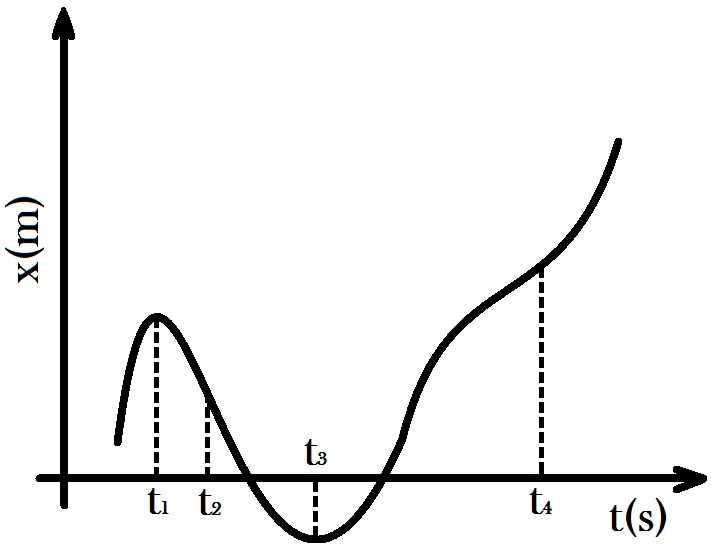
\includegraphics[width=0.45\textwidth]{yol_img1.jpg}
\end{center}



%%%%%%%%%%%%%%%%%%%%%%%%%%%%%%%%%%%
\begin{enumerate}
\item En $t_1$ la velocidad es 0 porque: \label{yolf-1}\\

\begin{enumerate}[(A)]
\item La pendiente de la recta tangente que es horizontal en ese punto es 0
\item  La curva ni crece ni decrece
\item  El cuerpo está en reposo
\item La aceleración es 0
\end{enumerate}


%%%%%%%%%%%%%%%%%%%%%%%%%%%%%%%%%%%
\newpage
\item En $t_2$ la velocidad es diferente de 0 pero negativa debido a:  \label{yolf-2}\\

\begin{enumerate}[(A)]
\item La pendiente de la recta tangente a la curva en ese punto es indeterminada
\item La pendiente de la recta tangente a la curva en ese punto es mayor que cero
\item  La pendiente de la recta tangente a la curva en ese punto es menor que cero
\item  La pendiente de la recta tangente a la curva en ese punto es igual a cero
\end{enumerate}

%%%%%%%%%%%%%%%%%%%%%%%%%%%%%%%%%%%
\item En $t_3$ la pendiente de la recta tangente a la curva es mayor que cero por tanto: \label{yolf-3}\\

\begin{enumerate}[(A)]
\item  La velocidad es indeterminada
\item  La velocidad es diferente de cero y positiva
\item La velocidad es diferente de cero y negativa
\item  La velocidad es igual a cero
\end{enumerate}

%%%%%%%%%%%%%%%%%%%%%%%%%%%%%%%%%%%
\newpage
\item  En $t_4$ la velocidad es igual a\label{yolf-4}\\

\begin{enumerate}[(A)]
\item La velocidad en $t_1$ porque las rectas tangentes a la curva en $t_1$ y en $t_4$ son paralelas y su pendiente es igual a cero
\item  La velocidad en $t_2$ porque las rectas tangentes a la curva en $t_2$ y en $t_4$ son perpendiculares y el producto de sus pendientes es -1
\item  La velocidad en $t_3$ porque las rectas tangentes a la curva en $t_3$ y en $t_4$ son horizontales
\item  Ninguno de los puntos marcados

\end{enumerate}

\subsubsection*{Las preguntas del \ref{yolf-5} al \ref{yolf-8} se contestan de acuerdo a la siguiente información:}

\noindent La figura muestra una gráfica de v contra t para el movimiento de un motociclista desde que parte del reposo y se mueve a lo largo de un camino en línea recta:

\begin{center}
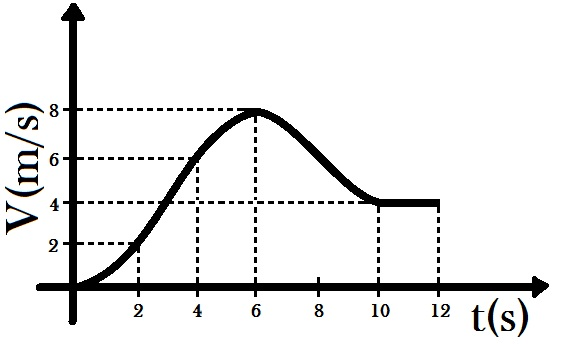
\includegraphics[width=0.45\textwidth]{yol_img2.jpg}
\end{center}

%%%%%%%%%%%%%%%%%%%%%%%%%%%%%%%%%%%
\item  La aceleración promedio puede ser calculada mediante la expresión: \label{yolf-5}\\

\begin{enumerate}[(A)]
\item  $a= v(0)-\frac{v(6)}{0-6}$
\item  $a= v(6)-\frac{v(0)}{6-0}$
\item  $a= \frac{0-6}{v(6)}-v(0)$
\item $a=\frac{6-0}{v(0)}-v(6)$

\end{enumerate}

%%%%%%%%%%%%%%%%%%%%%%%%%%%%%%%%%%%
\item El tiempo en el cual la aceleración tiene su mayor valor positivo y su valor en ese instante es: \label{yolf-6}\\

\begin{enumerate}[(A)]
\item  En $t=1$ y su valor es 1.1 $\frac{m}{s^2}$
\item  En $t=2$ y su valor es 2.2 $\frac{m}{s^2}$
\item  En $t=3$ y su valor es 1.3 $\frac{m}{s^2}$
\item  En $t=4$ y su valor es  2.2 $\frac{m}{s^2}$
\end{enumerate}

%%%%%%%%%%%%%%%%%%%%%%%%%%%%%%%%%%%
\item  La aceleración es 0 en $t=6$ y en $t=11$ porque: \label{yolf-7}\\

\begin{enumerate}[(A)]
\item  Las rectas tangentes a la curva son horizontales
\item  Las pendientes de las tangentes a la curva en esos puntos son iguales a 0
\item  Las pendientes son oblicuas y diferentes de 0
\item  Las opciones a y b son correctas
\end{enumerate}

%%%%%%%%%%%%%%%%%%%%%%%%%%%%%%%%%%%
\item  En $t=8$ la aceleración tiene un valor de -1.3$\frac{m}{s^2}$ , este valor es: \label{yolf-8}\\

\begin{enumerate}[(A)]
\item  El máximo valor positivo
\item  El máximo valor negativo
\item  El mínimo valor positivo
\item  El mínimo valor negativo
\end{enumerate}

\newpage
\subsubsection*{Las preguntas \ref{yolf-9} al \ref{yolf-12} se contestan de acuerdo a la siguiente información:}


\noindent Cada uno de los vectores de desplazamiento A y B mostrados en la figura tiene una magnitud de 3 metros

\begin{center}
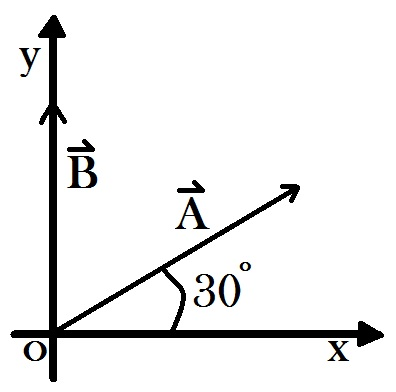
\includegraphics[width=0.3\textwidth]{yol_img3.jpg}
\end{center}
%%%%%%%%%%%%%%%%%%%%%%%%%%%%%%%%%%%
\item  La figura representa \label{yolf-9}\\

\begin{center}
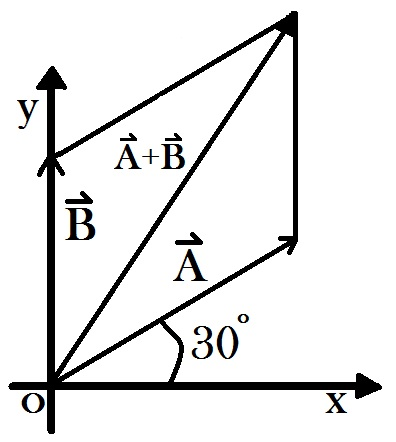
\includegraphics[width=0.3\textwidth]{yol_img4.jpg}
\end{center}

\begin{enumerate}[(A)]
\item  La suma de los vectores $\vec{A}$  y $\vec{B}$ por el método grafico
\item  La suma de los vectores $\vec{A}$  y $\vec{B}$ por el método del triangulo
\item  La suma de los vectores $\vec{A}$  y $\vec{B}$ por el método del paralelogramo
\item  La suma de los vectores $\vec{A}$  y $\vec{B}$ por el método de las componentes rectangulares
\end{enumerate}

%%%%%%%%%%%%%%%%%%%%%%%%%%%%%%%%%%%
\newpage
\item El vector $\vec{A}-\vec{B}$ \label{yolf-10}
\begin{center}
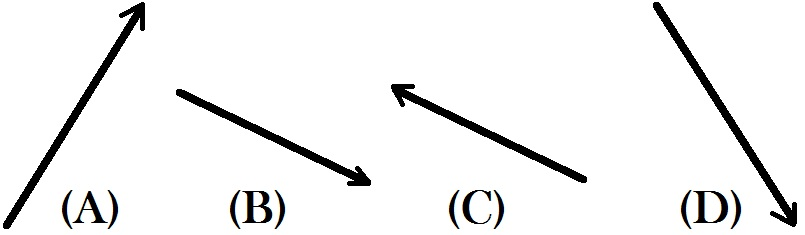
\includegraphics[width=0.45\textwidth]{yol_img5.jpg}
\end{center}

%%%%%%%%%%%%%%%%%%%%%%%%%%%%%%%%%%%
\item El vector $\vec{D}$ de la figura anterior representa \label{yolf-11}\\

\begin{enumerate}[(A)]
\item  $\vec{A}-\vec{B}$
\item  $\vec{A}+\vec{B}$
\item  $\vec{B}-\vec{A}$
\item  $\vec{A}-\vec{2B}$
\end{enumerate}

%%%%%%%%%%%%%%%%%%%%%%%%%%%%%%%%%%%
\item La magnitud del vector suma es  \label{yolf-12}\\

\begin{enumerate}[(A)]
\item  6 unidades en cualquier caso
\item  Mayor a 6 unidades si los vectores estuvieran sobre los ejes del plano
\item  Menor a 6 unidades
\item  Mayor a 6 unidades
\end{enumerate}

%%%%%%%%%%%%%%%%%%%%%%%%%%%%%%%%%%%
\item El trabajo se define como \label{yolf-13}\hrulefill\\
\_\hrulefill\\
\_\hrulefill\\
\_\hrulefill.


%%%%%%%%%%%%%%%%%%%%%%%%%%%%%%%%%%%
\item La relación entre el trabajo y la energía cinética se puede expresar como \label{yolf-14}\\

\begin{enumerate}[(A)]
\item  La suma de las energías cinéticas inicial y final
\item  La diferencia entre la energía cinética inicial y la energía cinética final
\item  La diferencia entre la energía cinética final y la energía cinética inicial
\item  El producto de las energías cinéticas inicial y final
\end{enumerate}

%%%%%%%%%%%%%%%%%%%%%%%%%%%%%%%%%%%
\item La potencia se define como \label{yolf-15}\hrulefill\\
\_\hrulefill\\
\_\hrulefill\\
\_\hrulefill.

%%%%%%%%%%%%%%%%%%%%%%%%%%%%%%%%%%%
\item La energía química de los alimentos se puede considerar como \label{yolf-16}\\

\begin{enumerate}[(A)]
\item  Energía cinética
\item  Energía potencial
\item  Energía potencial gravitacional
\item  Energía potencial elástica
\end{enumerate}

%%%%%%%%%%%%%%%%%%%%%%%%%%%%%%%%%%%
\item Con respecto al impulso se puede decir que \label{yolf-17}\\
\begin{enumerate}[(A)]
\item  Es el cambio en la velocidad porque al impulsarse la velocidad aumenta
\item  Es el cambio en la aceleración porque actúa la fuerza
\item  Es el cambio de la fuerza con relación al tiempo porque la fuerza es un vector
\item  Es el cambio en la cantidad de movimiento porque depende tanto d la masa como de la velocidad
\end{enumerate}

%%%%%%%%%%%%%%%%%%%%%%%%%%%%%%%%%%%
\item  Son elementos de una onda excepto \label{yolf-18}\\

\begin{enumerate}[(A)]
\item  Cresta ,valle y ciclo
\item  Difracción, interferencia y reflexión
\item  Amplitud, frecuencia y periodo
\item  Nodo, longitud de onda y velocidad de onda
\end{enumerate}

%%%%%%%%%%%%%%%%%%%%%%%%%%%%%%%%%%%
\item  La termodinámica es la rama de la física que \label{yolf-20}\hrulefill\\
\_\hrulefill\\
\_\hrulefill\\
\_\hrulefill.


%%%%%%%%%%%%%%%%%%%%%%%%%%%%%%%%%%%
\newpage
\item  Del sonido no se puede decir que  \label{yolf-19}\\

\begin{enumerate}[(A)]
\item  Es un fenómeno que involucra la propagación en forma de ondas elásticas
\item  Las ondas audibles producen oscilaciones en la presión del aire y las convierte en ondas mecánicas percibidas por el oído
\item  La propagación del sonido involucra transporte de energía y de materia
\item  Para que se genere un sonido es necesario que vibre alguna fuente
\end{enumerate}



%%%%%%%%%%%%%%%%%%%%%%%%%%%%%%%%%%%
\item   La primera ley de la termodinámica permite definir el calor como \label{yolf-21}\\

\begin{enumerate}[(A)]
\item  Un cambio en el trabajo sobre un sistema
\item  La energía necesaria que debe intercambiar un sistema para compensar las diferencias entre trabajo y energía interna
\item  Un cambio en la temperatura de un sistema
\item  Un cambio en la dirección en la que deben llevarse a cabo los procesos termodinámicos
\end{enumerate}
%%%%%%%%%%%%%%%%%%%%%%%%%%%%%%%%%%%
\item  Con respecto a las interacciones eléctricas no se puede concluir que. \label{yolf-22}\\

\begin{enumerate}[(A)]
\item  Son mucho más intensas que las interacciones gravitatorias
\item  Las cargas eléctricas pueden ser positivas o negativas
\item  Las interacciones entre las cargas eléctricas pueden ser atractivas o repulsivas
\item  La carga eléctrica constituye una medida de la estructura eléctrica de los átomos
\end{enumerate}

%%%%%%%%%%%%%%%%%%%%%%%%%%%%%%%%%%%
\item  La inercia es: \label{yolf-23}\hrulefill\\
\_\hrulefill\\
\_\hrulefill\\
\_\hrulefill.





%%%%%%%%%%%%%%%%%%%%%%%%%%%%%%%%%%%
\item   El voltaje se relaciona con: \label{yolf-25}\hrulefill\\
\_\hrulefill\\
\_\hrulefill\\
\_\hrulefill.


\newpage
%%%%%%%%%%%%%%%%%%%%%%%%%%%%%%%%%%%
\item   Un fluido se caracteriza por: \label{yolf-24}\\

\begin{enumerate}[(A)]
\item  Ser un medio que se mueve
\item  Su incapacidad para resistir esfuerzos cortantes
\item  Carecer de forma definida
\item  La opción b y c son correctas
\end{enumerate}

%%%%%%%%%%%%%%%%%%%%%%%%%%%%%
\end{enumerate}
%%%%%%%%%%%%%%%%%%%%%%%%%%%%%5

